% % % % % % % % % % % % % % % % % % % % % % % % % % % % % % % % % % % %
%\documentclass[letter]{sig-alternate-05-2015}
\documentclass[letter]{vldb}
% % % % % % % % % % % % % % % % % % % % % % % % % % % % % % % % % % % %
\usepackage[tight,footnotesize]{subfigure}
\setlength{\paperheight}{11in}
\setlength{\paperwidth}{8.5in}
%\usepackage[
%  pass,% keep layout unchanged
%  % showframe,% show the layout
%]{geometry}

%\usepackage{times}
% % % % % % % % % % % % % % % % % % % % % % % % % % % % % % % % % % % %
\usepackage{booktabs, multicol, multirow}
\usepackage[acronym,nomain]{glossaries}
\usepackage[inline]{enumitem}
\usepackage{algorithm}
\usepackage{algorithmicx}
\usepackage{algpseudocode}
\usepackage{amsmath}
\usepackage{subfigure}
\usepackage{grffile}
\usepackage{tabularx}
\usepackage{colortbl}
\usepackage{hhline}
\usepackage{hyperref}
\usepackage[flushleft]{threeparttable}
\usepackage{booktabs,caption,fixltx2e}
\usepackage{balance}
\newcommand{\bs}{\boldsymbol}
\renewcommand{\mathbf}[1]{{\boldsymbol #1}}
\hypersetup{
	colorlinks   = true,
	citecolor    = blue,
	linkcolor    = blue,
}
\usepackage{graphicx}
% % % % % % % % % % % % % % % % % % % % % % % % % % % % % % % % % % % %




\newtheorem{theorem}{Theorem}[section]
\newtheorem{lemma}[theorem]{Lemma}
\newtheorem{proposition}[theorem]{Proposition}
\newtheorem{corollary}[theorem]{Corollary}




%%%%%%%%%%%%%%%%%%%%%%%%%%%%%%%%%%%%%%%%%%%%%%%%%%

% % % % % % % % % % % % % % % % % % % % % % % % % % % % % % % % % % % % new commands % % %
\usepackage[colorinlistoftodos,prependcaption,textsize=tiny]{todonotes}
%
% Convenience commands for the paper editing process
%
\newcommand{\GC}[1]{{\textbf{\color{red}[GC: #1]}}}
\newcommand{\PJ}[1]{{\textbf{\color{blue}[PJ: #1]}}}
\newcommand{\GCOMMENT}[1]{{\em {\color{red}[GC REMOVE: #1]}}} % GC: I want to use the comment package, but this overrides it so I changed it
\newcommand{\fixed}[1]{{\textbf{\color{blue}[#1]}}}


%
% Convenience commands for references
%
\newcommand{\secref}[1]{Section~\ref{sec:#1}}
\newcommand{\tabref}[1]{Table~\ref{tab:#1}}
\newcommand{\figref}[1]{Figure~\ref{fig:#1}}
\newcommand{\quotes}[1]{``#1''}

\newcommand{\argmin}{\arg\!\min}
\newcommand{\argmax}{\arg\!\max}


\newtheorem{definition}{Definition}

\renewcommand{\algorithmicrequire}{\textbf{Input:}}
\renewcommand{\algorithmicensure}{\textbf{Output:}}

\newcolumntype{g}{>{\columncolor{blue!25}}c}

% % % % % % % % % % % % % % % % % % % % % % % % % % % % % % % % % % % %

% % % % % % % % % % % % % % % % % % % % % % % % % % % % % % % % % % % %
% Acronym definitions
%\newacronym{sps}{SPS}{stream processing system}
%\newacronym{pe}{PE}{processing element}
%\newacronym{dag}{DAG}{Directed Acyclic Graph}

% % % % % % % % % % % % % % % % % % % % % % % % % % % % % % % % % % % %



% Generate the glossary
\makeglossaries

\begin{document}

\title{Supplementary material for: \\ Transfer Learning for Optimal Configuration \\ of Big Data Software}
\maketitle


In this extra material, we briefly describe additional details about the experimental setting and complementary results that were not included in the main text. 

\section{Further Details on Settings}

\subsection{Code: {\sf \large TL4CO} \& {\sf \large BO4CO}}

{\noindent \small \url{https://github.com/dice-project/DICE-Configuration-BO4CO}}

{\noindent \small \url{https://github.com/dice-project/DICE-Configuration-TL4CO}}


\subsection{Instructions for Storm Deployment}
Since it is non trivial, we documented here how to deploy Storm on EC2, Azure and OpenNebula:

{\noindent \small \url{https://gist.github.com/pooyanjamshidi/e3570c275037043944fe}}




\subsection{Configuration Parameters}

{\small 
The Apache Storm parameters (cf. Table \ref{tab:configuration-parameters}): 
\begin{itemize}
	\setlength\itemsep{0em}
	\item {\sf max\_spout (topology.max.spout.pending)}. The maximum number of tuples that can be pending on a spout.
	\item {\sf spout\_wait (topology.sleep.spout.wait.strategy.time.ms)}. Time in ms the {\sf SleepEmptyEmitStrategy} should sleep.
	\item  {\sf netty\_min\_wait (storm.messaging.netty.min\_wait\_ms)}. The min time {\sf netty} waits to get the control back from OS. 
	\item {\sf spouts, splitters, counters, bolts}. Parallelism level. 
	\item {\sf heap}. The size of the worker heap.
	\item  {\sf buffer\_size (storm.messaging.netty.buffer\_size)}. The size of the transfer queue.
	\item {\sf emit\_freq (topology.tick.tuple.freq.secs)}. The frequency at which tick tuples are received.
	\item {\sf top\_level}. The length of a linear topology. 
	\item {\sf message\_size, chunk\_size}. The size of tuples and chunk of messages sent across PEs respectively.
\end{itemize}


The Apache Cassandra parameters (cf. Table \ref{tab:configuration-parameters}): 
\begin{itemize}
		\setlength\itemsep{0em}
	\item {\sf trickle\_fsync}: when enabled it forces OS to flush the write buffer at a regular time. 
	\item {\sf auto\_snapshot}: enables the system to take snapshots, avoiding to lose data during truncation or table drop. 
	\item {\sf concurrent\_reads}: number of threads dedicated to the read operations.
	\item {\sf concurrent\_writes}: number of threads dedicated to the write operations. 
	\item {\sf file\_cache\_size\_in\_mb}: the memory used as reading buffers.
	\item {\sf concurrent\_compactors}:  number of threads dedicated to the compaction process of the data on the disk.
\end{itemize}
}

\subsection{Datasets}

\begin{table}[h!]
	\centering
	\caption{\small Experimental datasets, note that this is the complete set of datasets that we experimentally collected over the course of 3 month of 6 different cloud infrastructures. We only have shown part of this in the paper.} %The merit function indicates the significant is the set of strongly-interacting parameters that best explains the data. 
	\label{tab:configuration-parameters}
	\resizebox{\columnwidth}{!}{%
		\begin{threeparttable}
			\begin{tabular}{@{}lllgc@{}}
				\toprule
				&\textbf{Dataset} & \multicolumn{1}{c}{\textbf{Parameters}}                                                                                       & \multicolumn{1}{c}{\textbf{Size}} & \multicolumn{1}{c}{\textbf{Testbed}}                                                                             \\ \midrule
				1  & {\sf wc(6D) }               & \begin{tabular}[c]{@{}l@{}}{\sf 1-spouts: \textcolor{blue}{\{1,3\}},}\\ {\sf 2-max\_spout: \textcolor{blue}{\{1,2,10,100,1000,10000\}}, }\\ {\sf 3-spout\_wait:\textcolor{blue}{\{1,2,3,10,100\},}}\\ {\sf 4-splitters:\textcolor{blue}{\{1,2,3,6\}},}\\ {\sf 5-counters:\textcolor{blue}{\{1,3,6,12\}},} \\ {\sf 6-netty\_min\_wait:\textcolor{blue}{\{10,100,1000\}}} \end{tabular}                      & 2880 & C1                 \\ \midrule
				2  & {\sf sol(6D) }             & \begin{tabular}[c]{@{}l@{}}{\sf 1-spouts:\textcolor{blue}{\{1,3\}},} \\ {\sf 2-max\_spout:\textcolor{blue}{\{1,10,100,1000,10000\}},} \\ {\sf 3-top\_level:\textcolor{blue}{\{2,3,4,5\}},} \\ {\sf 4-netty\_min\_wait:\textcolor{blue}{\{10,100,1000\}},} \\ {\sf 5-message\_size: \textcolor{blue}{\{10,100,1e3,1e4,1e5,1e6\}},} \\ {\sf 6-bolts: \textcolor{blue}{\{1,2,3,6\}}} \end{tabular}                          & 2866 & C2                          \\ \midrule
				3  & {\sf rs(6D) }           & \begin{tabular}[c]{@{}l@{}}{\sf 1-spouts:\textcolor{blue}{\{1,3\}},} \\ {\sf 2-max\_spout:\textcolor{blue}{\{10,100,1000,10000\}}, }\\ {\sf 3-sorters:\textcolor{blue}{\{1,2,3,6,9,12,15,18\}},} \\ {\sf 4-emit\_freq:\textcolor{blue}{\{1,10,60,120,300\}},}\\ {\sf 5-chunk\_size:\textcolor{blue}{\{1e5,1e6,2e6,1e7\}},} \\ {\sf 6-message\_size:\textcolor{blue}{\{1e3,1e4,1e5\}}} \end{tabular}                                    & 3840 & C3              \\ \midrule
				4  & {\sf wc(3D)}            & \begin{tabular}[c]{@{}l@{}}{\sf 1-max\_spout:\textcolor{blue}{\{1,10,100,1e3, 1e4,1e5,1e6\}},} \\ {\sf 2-splitters:\textcolor{blue}{\{1,2,3,4,5,6\}},} \\ {\sf 3-counters:\textcolor{blue}{\{1,2,3,4,5,6,7,8,9,10,11,12,13,14,15,16,17,18\}}} \end{tabular}                                                                             & 756 & C4                            \\ \midrule
				5  & {\sf wc+rs }          & \begin{tabular}[c]{@{}l@{}}{\sf 1-max\_spout:\textcolor{blue}{\{1,10,100,1e3, 1e4,1e5,1e6\}},} \\ {\sf 2-splitters:\textcolor{blue}{\{1,2,3,6\}},} \\ {\sf 3-counters:\textcolor{blue}{\{1,3,6,9,12,15,18\}}} \end{tabular}                                                                              & 196 & C4                                \\ \midrule
				6  & {\sf wc+sol }         & \begin{tabular}[c]{@{}l@{}}{\sf 1-max\_spout:\textcolor{blue}{\{1,10,100,1e3, 1e4,1e5,1e6\}},} \\ {\sf 2-splitters:\textcolor{blue}{\{1,2,3,6\}},} \\ {\sf 3-counters:\textcolor{blue}{\{1,3,6,9,12,15,18\}}} \end{tabular}                                                                                  & 196 & C4                              \\ \midrule
				7  & {\sf wc+wc }        & \begin{tabular}[c]{@{}l@{}}{\sf 1-max\_spout:\textcolor{blue}{\{1,10,100,1e3, 1e4,1e5,1e6\}},} \\ {\sf 2-splitters:\textcolor{blue}{\{1,2,3,6\}},} \\ {\sf 3-counters:\textcolor{blue}{\{1,3,6,9,12,15,18\}}} \end{tabular}                                                                       & 196 & C4                                \\ \midrule
				8  & {\sf wc(5D)}            & \begin{tabular}[c]{@{}l@{}}{\sf 1-spouts:\textcolor{blue}{\{1,2,3\}},} \\ {\sf 2-splitters:\textcolor{blue}{\{1,2,3,6\}},} \\ {\sf 3-counters:\textcolor{blue}{\{1,2,3,6,9,12\}},} \\ {\sf 4-buffer-size:\textcolor{blue}{\{256k,1m,5m,10m,100m\}},} \\ {\sf 5-heap:\textcolor{blue}{\{``-Xmx512m", ``-Xmx1024m", ``-Xmx2048m"\}}} \end{tabular}                                                                     & 1080 & C5                            \\ \midrule
				9  & {\sf wc-c1}        & \begin{tabular}[c]{@{}l@{}}{\sf 1-spout\_wait:\textcolor{blue}{\{1,2,3,4,5,6,7,8,9,10,100,1e3,1e4\}},} \\ {\sf 2-splitters:\textcolor{blue}{\{1,2,3,4,5,6\}},}\\ {\sf 3-counters:\textcolor{blue}{\{1,2,3,4,5,6,7,8,9,10,11,12,13,14,15,16,17,18\}}} \end{tabular}                                                                               & 1343 & C1                          \\ \midrule
				10 & {\sf wc-c3}      & \begin{tabular}[c]{@{}l@{}}{\sf 1-spout\_wait:\textcolor{blue}{\{1,2,3,4,5,6,7,8,9,10,100,1e3,1e4,6e4\}},} \\ {\sf 2-splitters:\textcolor{blue}{\{1,2,3,4,5,6\}},}\\ {\sf 3-counters:\textcolor{blue}{\{1,2,3,4,5,6,7,8,9,10,11,12,13,14,15,16,17,18\}}} \end{tabular}                                                              & 1512 & C3 \\  \midrule
				\begin{tabular}[c]{@{}l@{}}11 \\ \\ 12\end{tabular} & \begin{tabular}[c]{@{}l@{}} {\sf cass-10 } \\ \\ {\sf cass-20 }\end{tabular}      & \begin{tabular}[c]{@{}l@{}}{\sf 1-trickle\_fsync:\textcolor{blue}{\{false,true\}},} \\ {\sf 2-auto\_snapshot:\textcolor{blue}{\{false,true\}},} \\ {\sf 3-con.\_reads:\textcolor{blue}{\{16,24,32,40\}},} \\ {\sf 4-con.\_writes:\textcolor{blue}{\{16,24,32,40\}},} \\ {\sf 5-file\_cache\_size\_in\_mb:\textcolor{blue}{\{256,384,512,640\}},}\\ {\sf 6-con.\_compactors:\textcolor{blue}{\{1,3,5,7\}}} \end{tabular}                                                              & 1024 & C6 \\
				\bottomrule
			\end{tabular}
		\end{threeparttable}}
	\end{table}


\newpage

\subsection{Benchmark Settings}

\begin{table}[h!]
	\centering
	\caption{Cluster specification}
	%\vspace{-1em}
	\label{tab:cluster-specification}
	\resizebox{\columnwidth}{!}{%
		\begin{tabular}{@{}cl@{}}
			\toprule
			\textbf{Cluster} & \multicolumn{1}{c}{\textbf{Specification}}                                                                                   \\ \midrule
			C1               & \begin{tabular}[c]{@{}l@{}}OpenNebula, 3 Sup, 1 ZK, 1 Nimbus, N: (1CPU, 4GB Mem)\end{tabular}                               \\ \midrule
			C2               & \begin{tabular}[c]{@{}l@{}}EC2, 3 Sup, 1 ZK, 1 Nimbus, N: m1.medium (1 CPU, 3.75GB)\end{tabular}                          \\ \midrule
			C3               & \begin{tabular}[c]{@{}l@{}}OpenNebula, 3 Sup: (3CPU,6GB Mem), 1 ZK: (1CPU,4GB Mem),\\ 1 Nimbus: (2CPU,4GB Mem)\end{tabular} \\ \midrule
			C4               & \begin{tabular}[c]{@{}l@{}}EC2, 3 Sup, 1 ZK, 1 Nimbus, N: m3.large (2CPU, 7.5GB)\end{tabular}                             \\ \midrule
			C5               & \begin{tabular}[c]{@{}l@{}}Azure, 3 Sup: Standard\_D1(1CPU, 3.5GB) , 1 ZK, 1 Nimbus, \\ N: Standard\_A1(1CPU, 1.75GB) \end{tabular}                         \\ \midrule
			C6               & \begin{tabular}[c]{@{}l@{}}OpenNebula, 1 N(4CPU, 4GB, 2 Disks) \end{tabular}                         \\ 
			\bottomrule
		\end{tabular}
	}
\end{table}



\begin{table}[h!]
	\centering
	\caption{Cassandra benchmark specification.}
	\label{tab:ycsb}
	\resizebox{0.6\columnwidth}{!}{%
		\begin{tabular}{| l | g |}
			\hline
			\textbf{Parameter} & \textbf{Value} \\ \hline
			Column family fields & 10 \\ \hline
			Column family data size & 1K \\ \hline
			Read requests & 50\% \\ \hline
			Update requests & 50\% \\ \hline
			Read all fields & yes \\ \hline
			Requests distribution & uniform \\ \hline
			YCSB threads & 2 \\ \hline
		\end{tabular}}
	\end{table}

\begin{figure}[h!]
	\begin{center}
		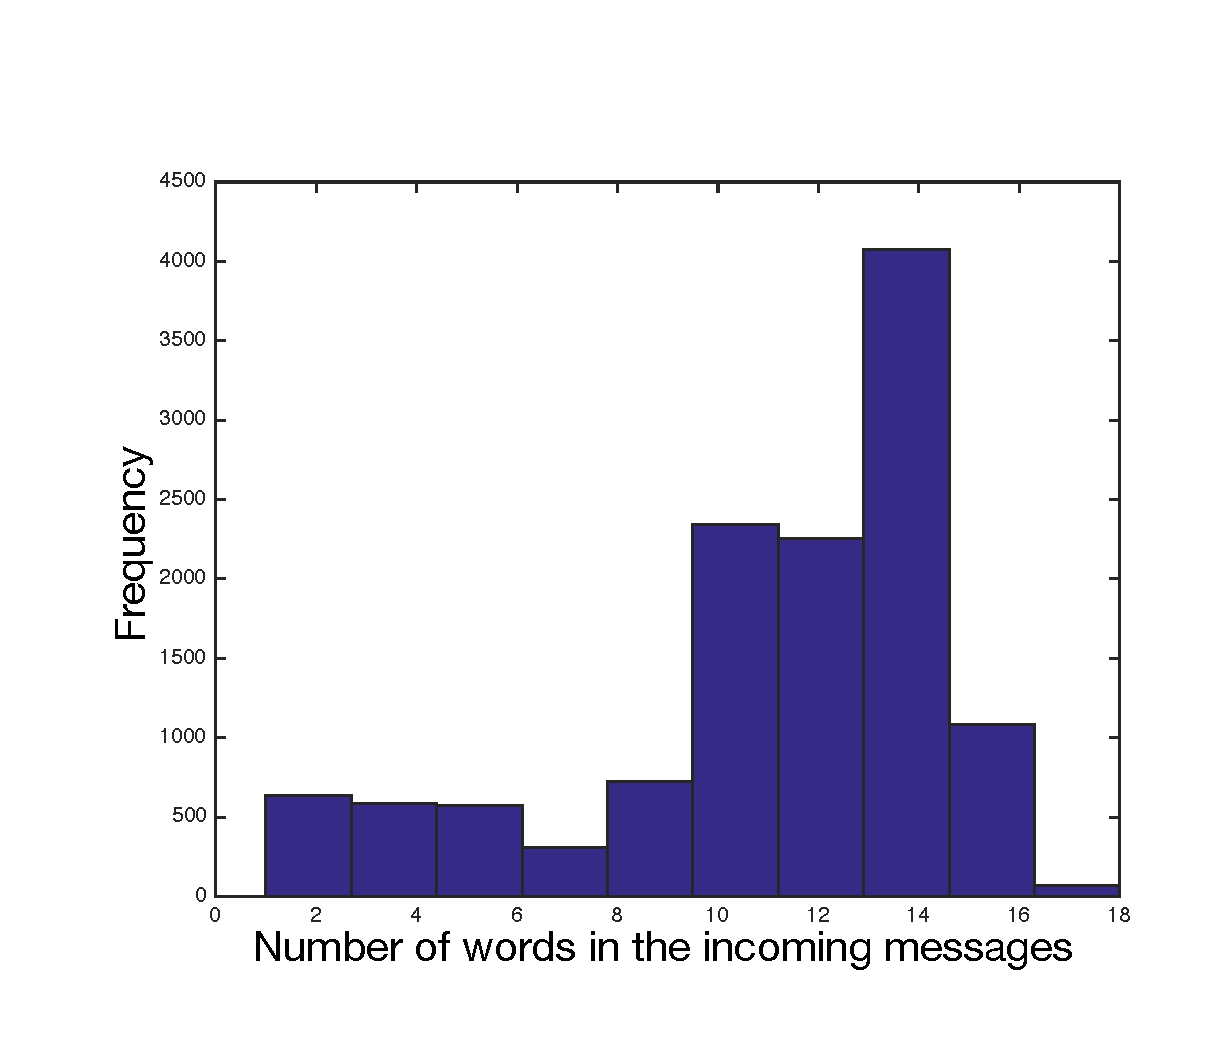
\includegraphics[width=0.7\columnwidth]{figures/hist-arrival-lenght1}
		\caption{{\sf WordCount} workload (arrival rate). Note that for {\sf RollingSort} and {\sf SOL} experiments the size of the incoming messages are set to 100. The message itself is randomely created by {\sf StringBuilder} procedure which append 100 integer number between 1-9 randomly.}
		\label{fig:wc-arrival}
	\end{center}
\end{figure}


%{\noindent \large \textbf{Apache Storm Architecture}.}

\subsection{Apache Storm Architecture}

\begin{figure}[h!]
	\begin{center}
		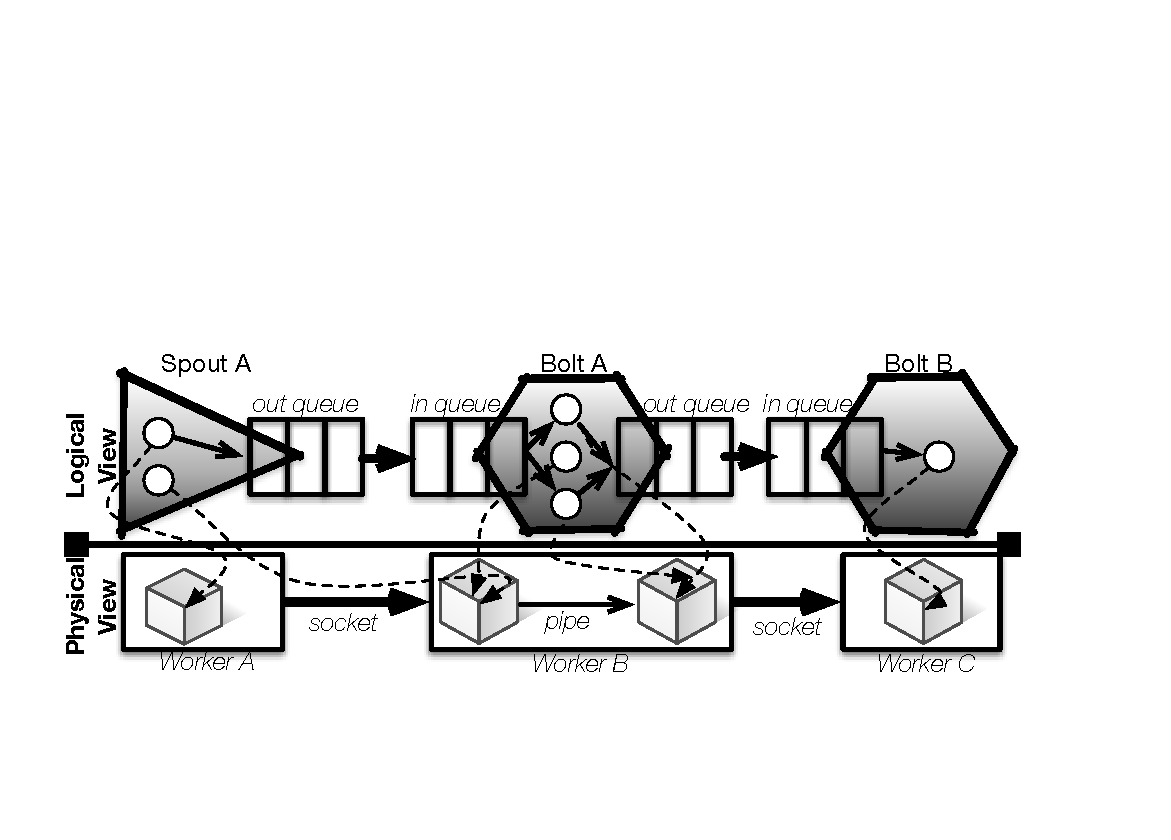
\includegraphics[width=\columnwidth]{figures/system-model}
		\caption{System model of a SPS with three worker nodes.}
		\label{fig:system-model}
	\end{center}
\end{figure}

\begin{figure}[h!]
	\begin{center}
		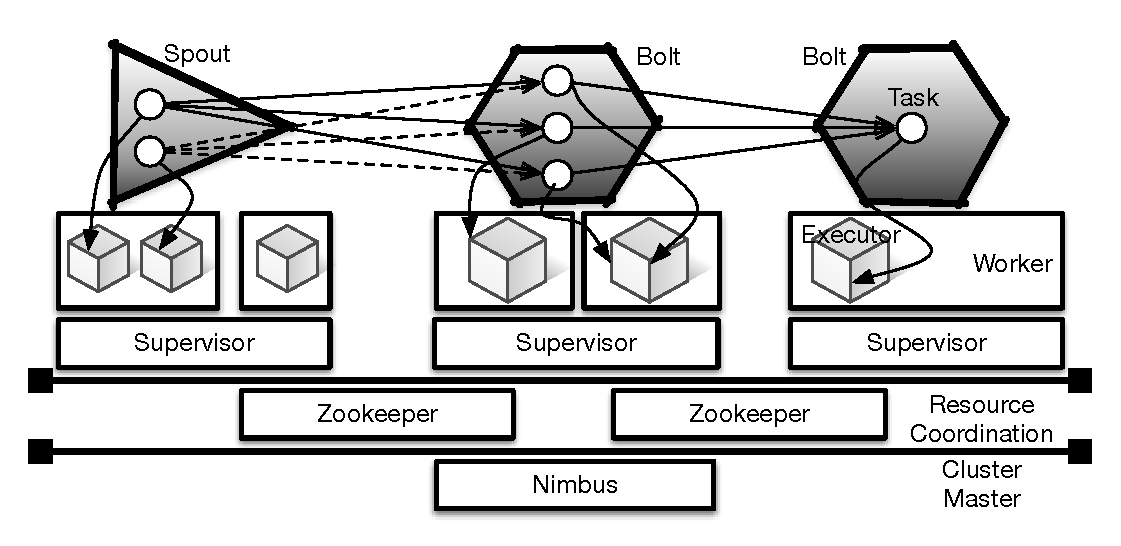
\includegraphics[width=0.9\columnwidth]{figures/storm-architecture}
					\vspace{-1em}
		\caption{Apache Storm architecture.}
		\label{fig:storm-arch}
	\end{center}
\end{figure}


\begin{figure}[h!]
	\begin{center}
		\vspace{-2em}
		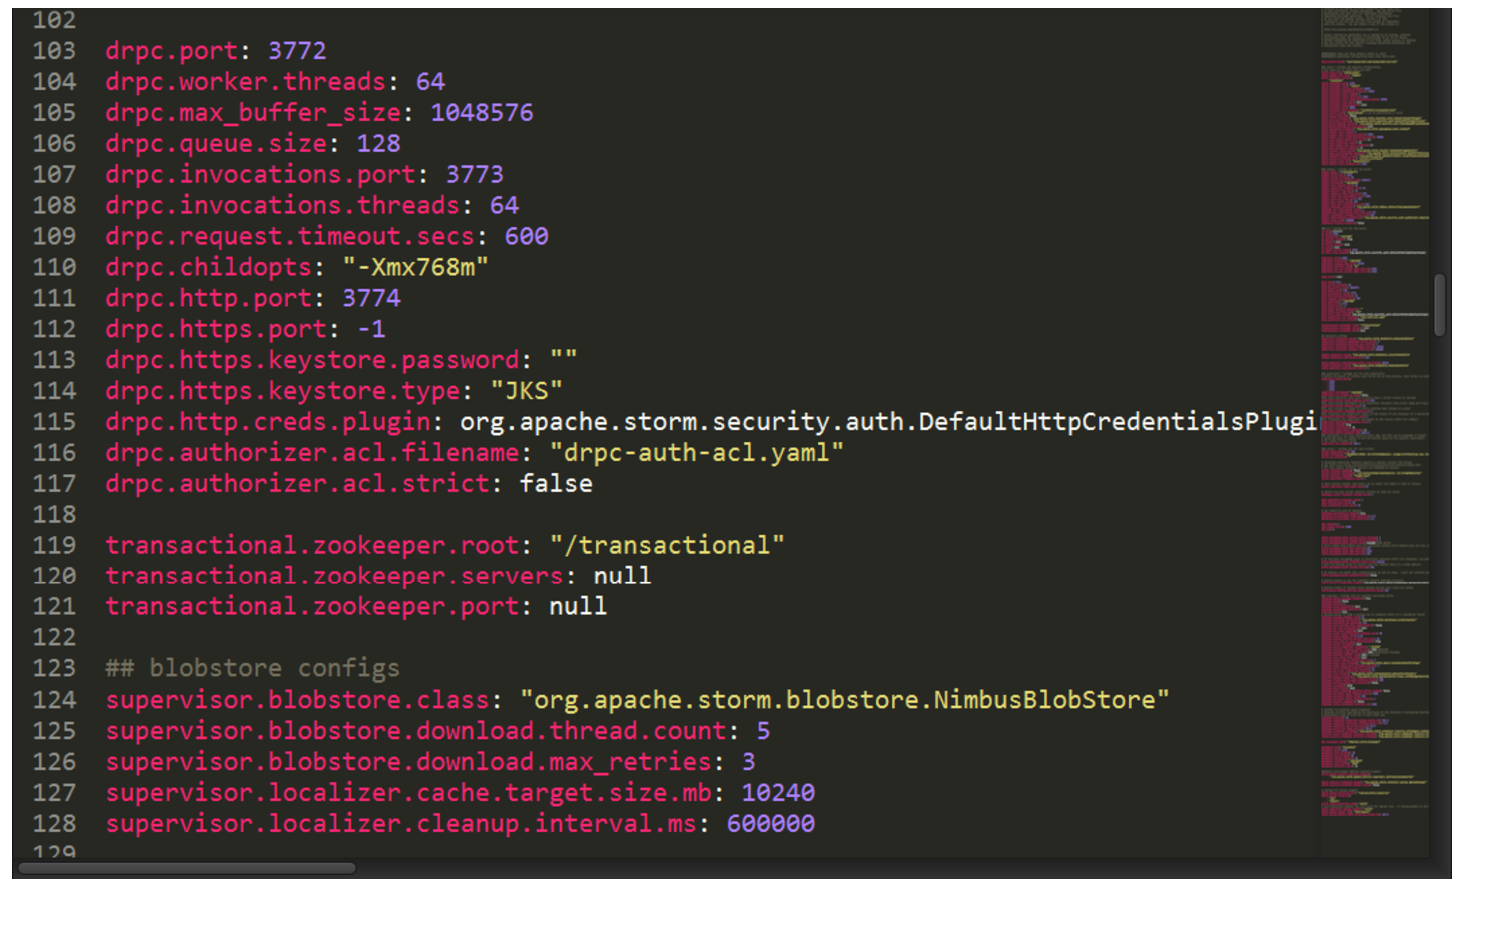
\includegraphics[width=1.1\columnwidth]{figures/config-params}
			\vspace{-3em}
		\caption{An example of a {\sf YAML} file for Storm containing configuration parameters that we automatically change.}
		\vspace{-2em}
		\label{fig:yaml-example}
		
	\end{center}
\end{figure}


\newpage
%{\noindent \large \textbf{Response Surfaces: {\sf Branin} and {\sf Cassandra}.}}

\subsection{Additional Response Surfaces}

\begin{figure}[h!] 
	\begin{center}
		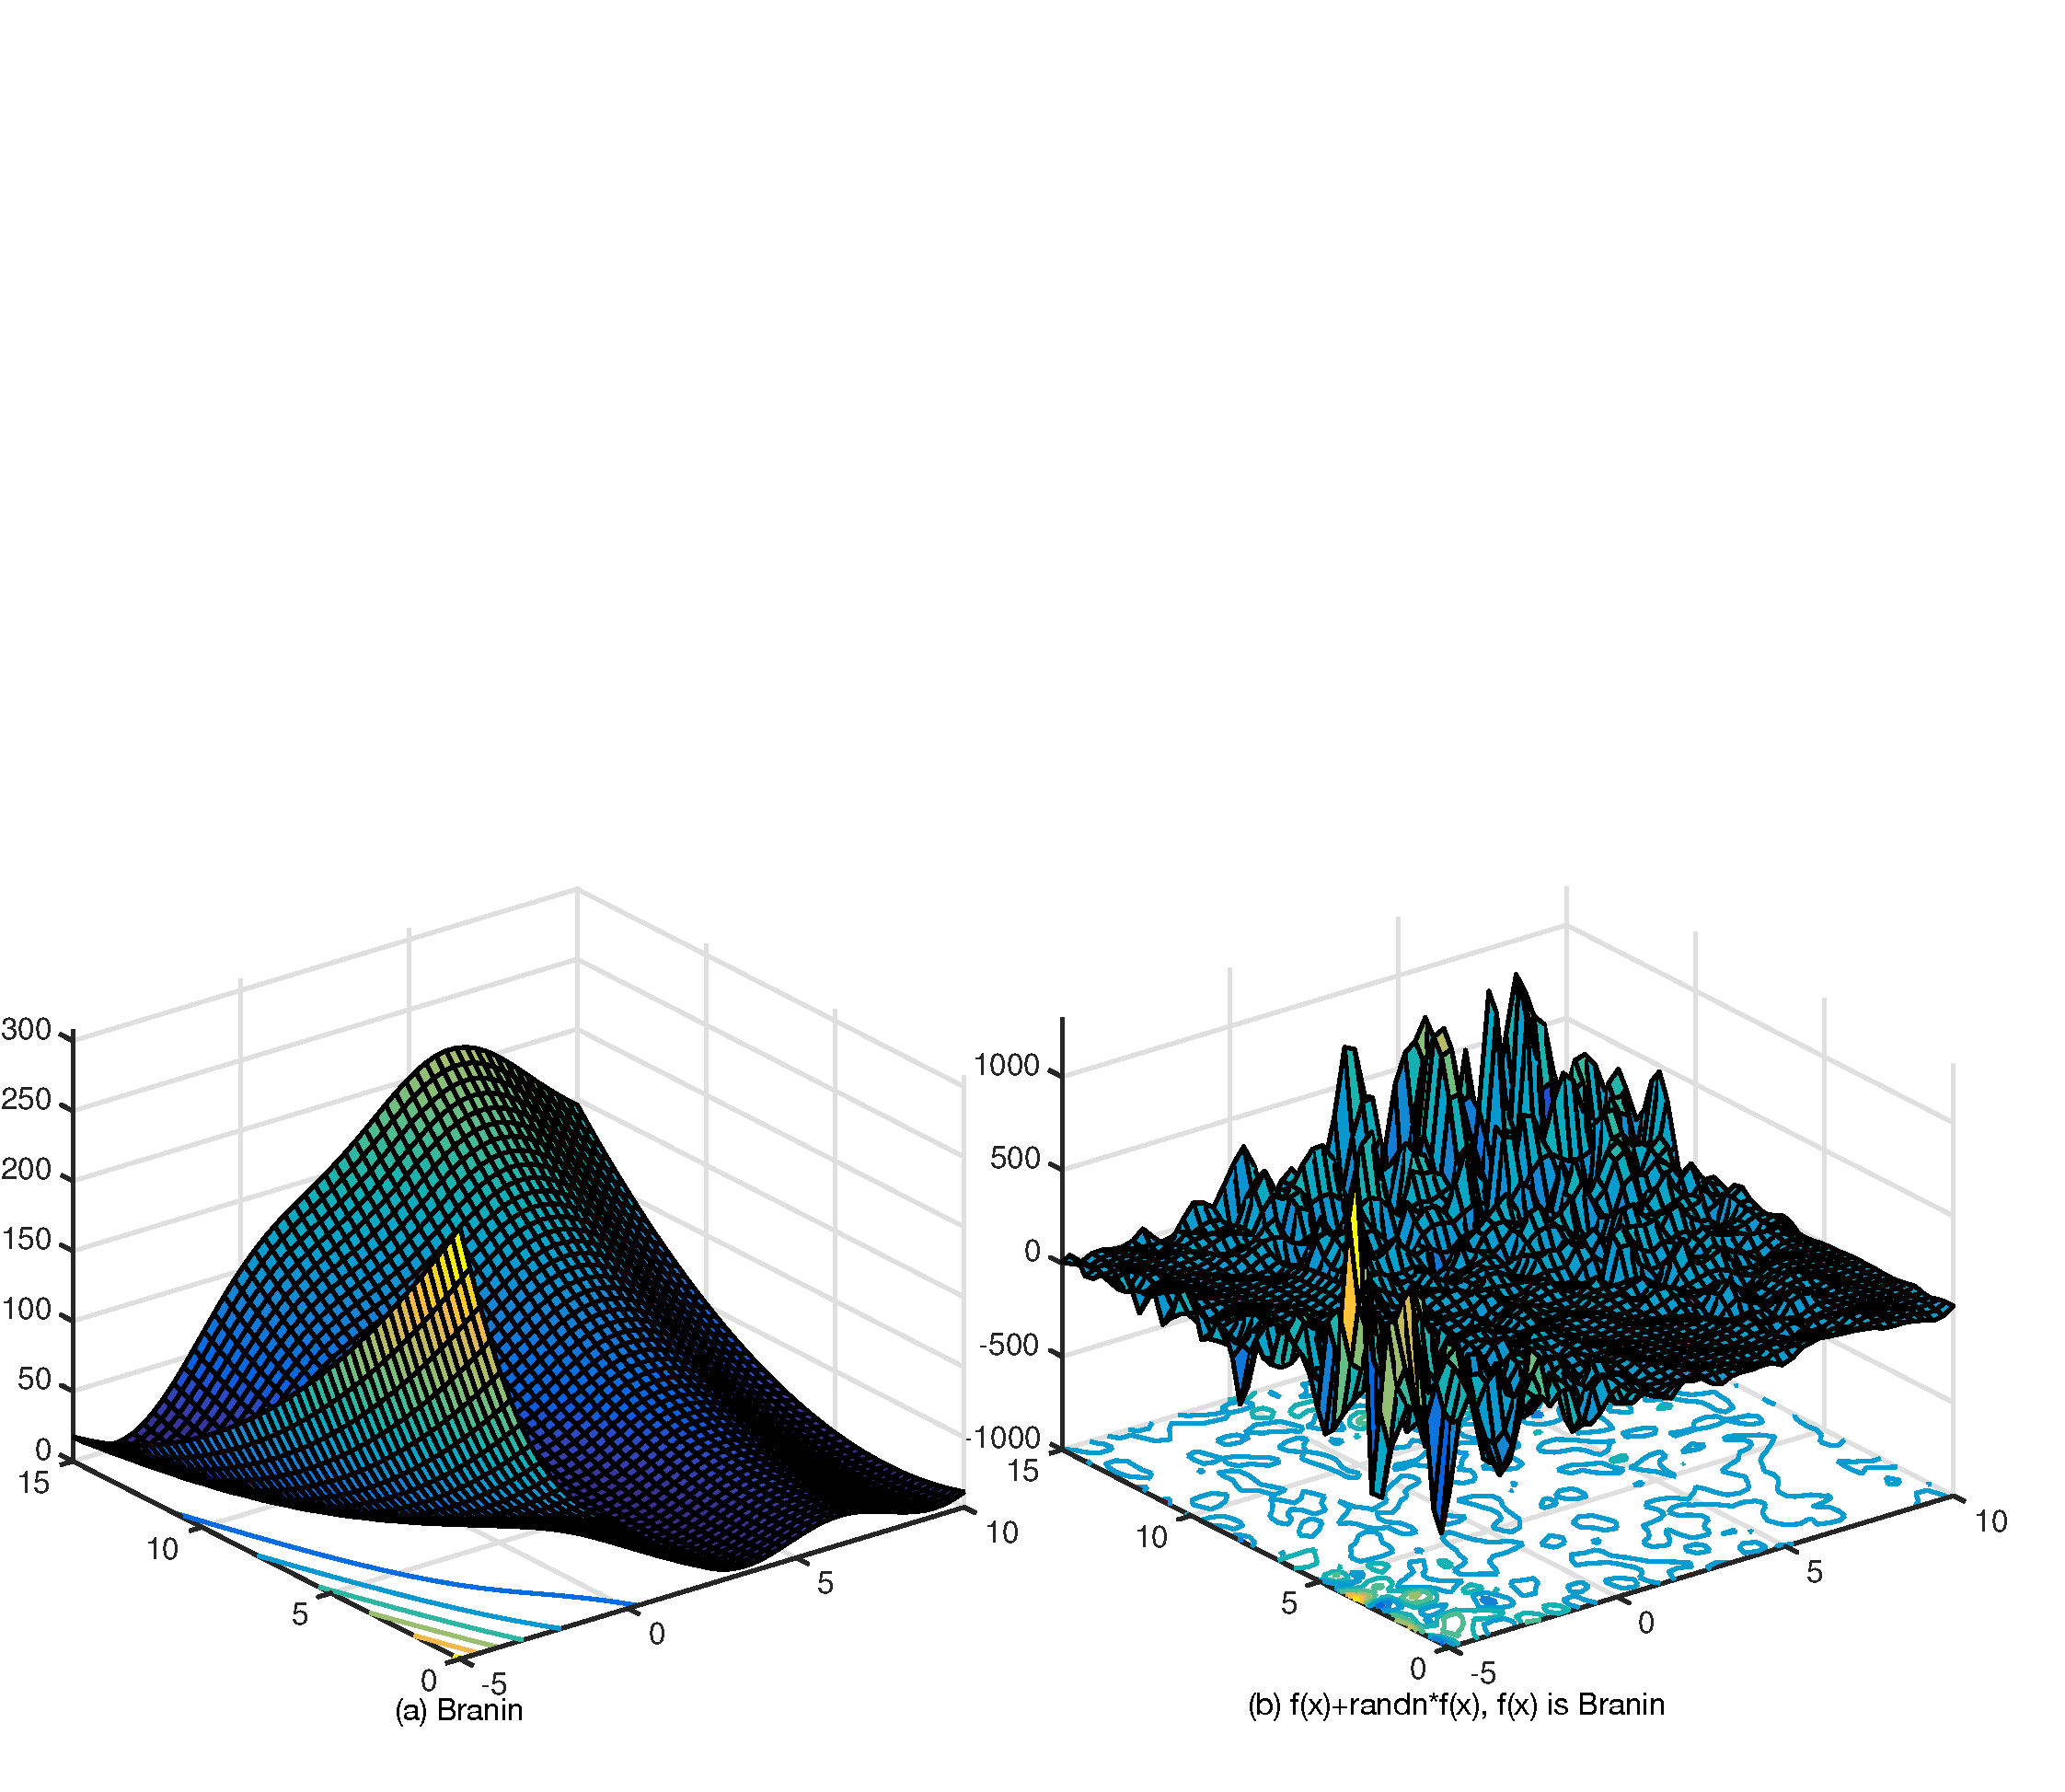
\includegraphics[width=\columnwidth]{figures/dixon-branin-randn}
		\caption{(a) {\sf Branin(2D)}, (b) $f(\mathbf{x})+randn\times f(\mathbf{x})$.}
		\label{fig:dixon-rand-surface}
	\end{center}
\end{figure}

\begin{figure}[h!]
	\begin{center}
		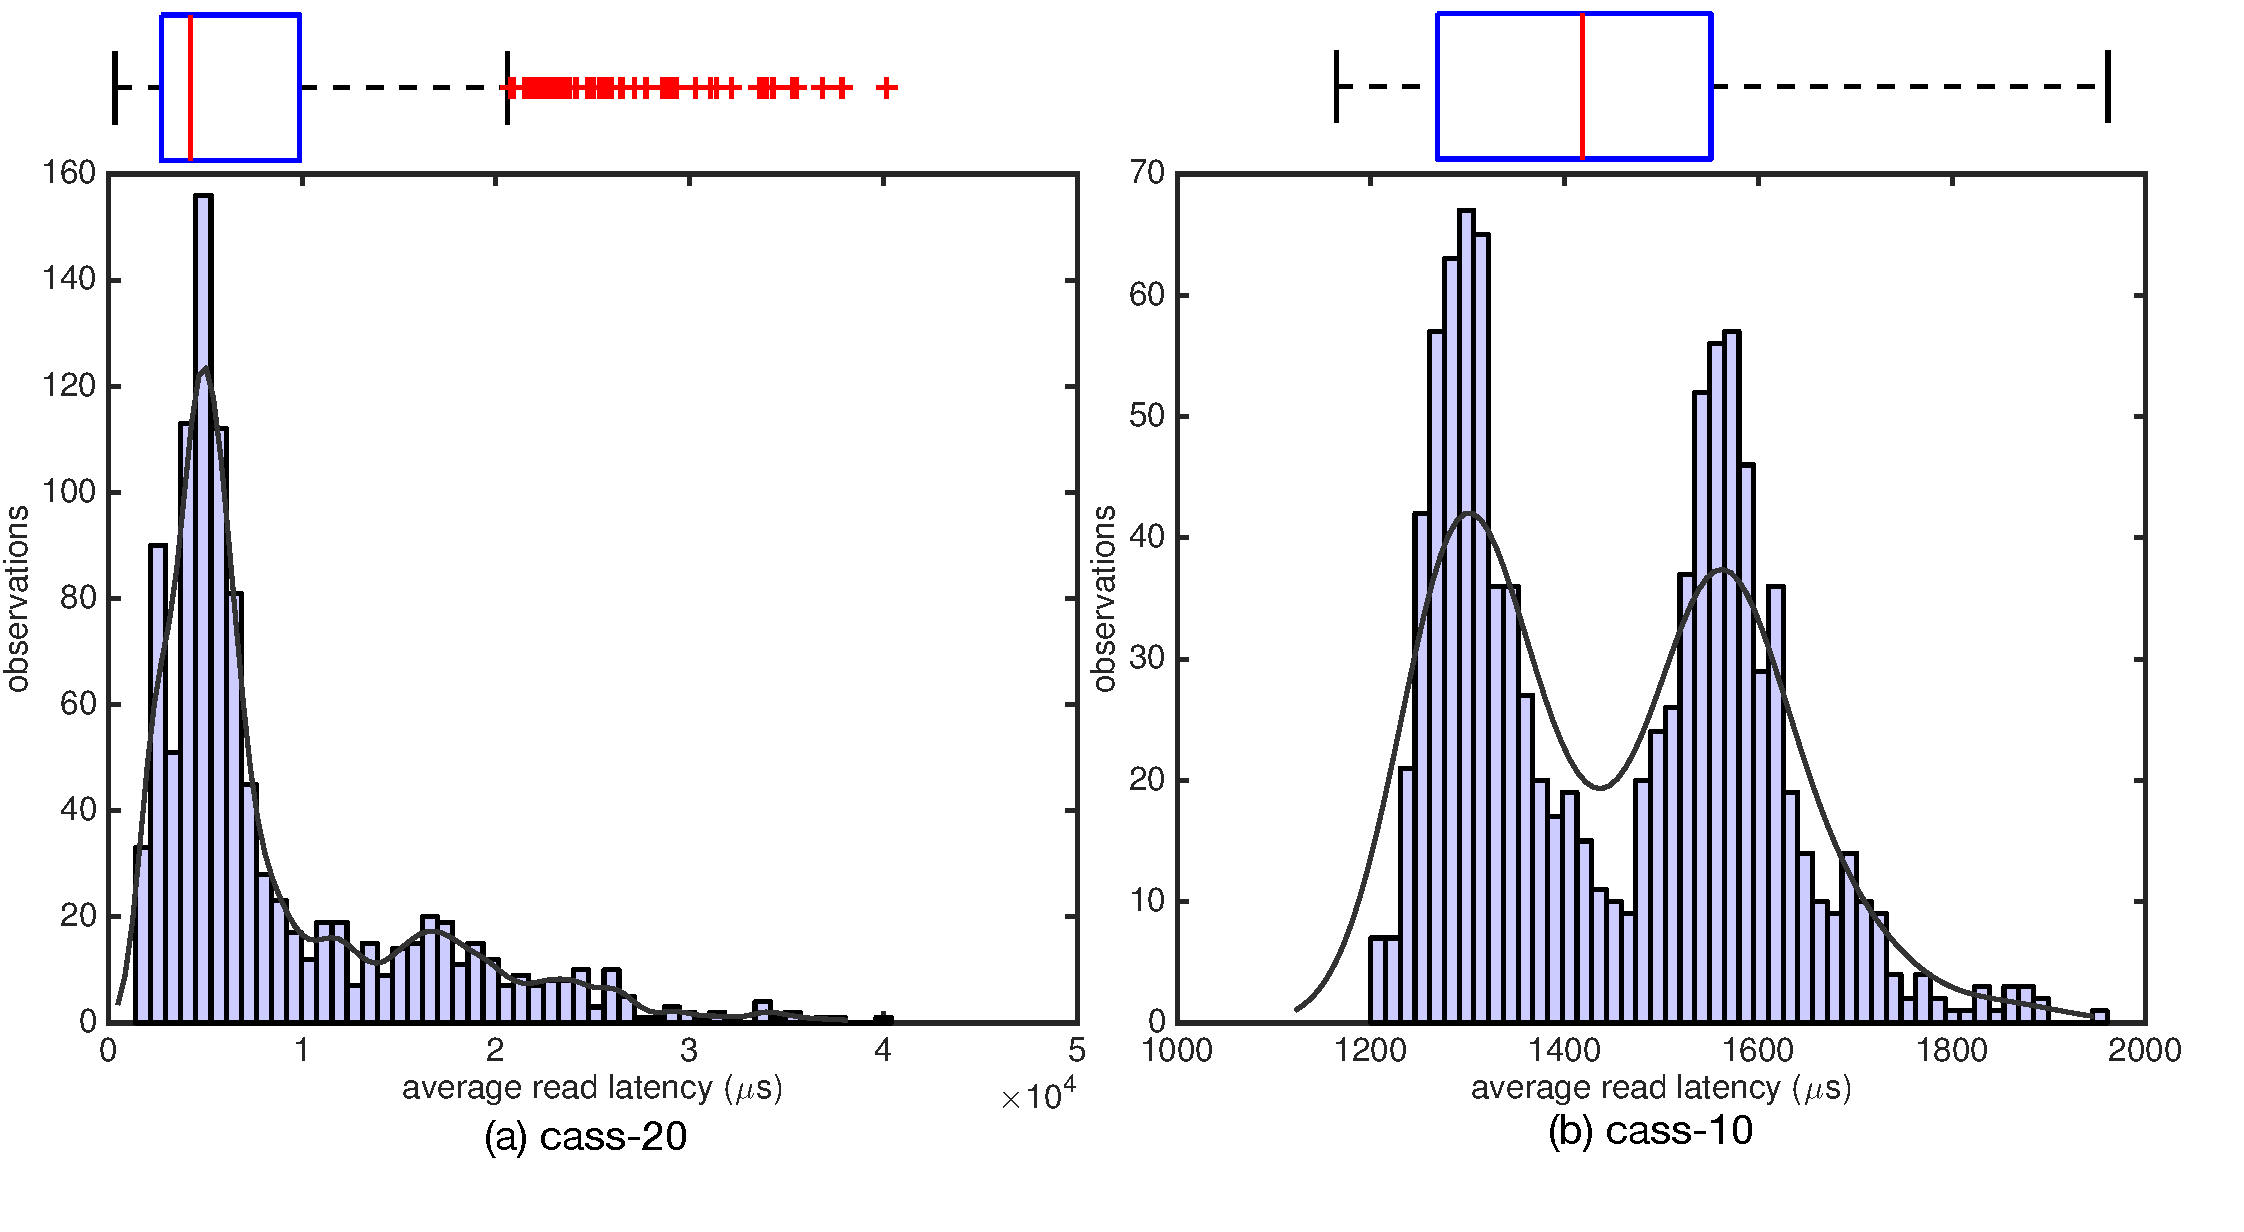
\includegraphics[width=1.1\columnwidth]{figures/109-138-read-hist-boxplot}
		\caption{Average latency for (a) {\sf cass-20}, (b) {\sf cass-10}.}
		\label{fig:read-latency-hist}
	\end{center}
\end{figure}

\begin{figure*}[t]
	\begin{center}
		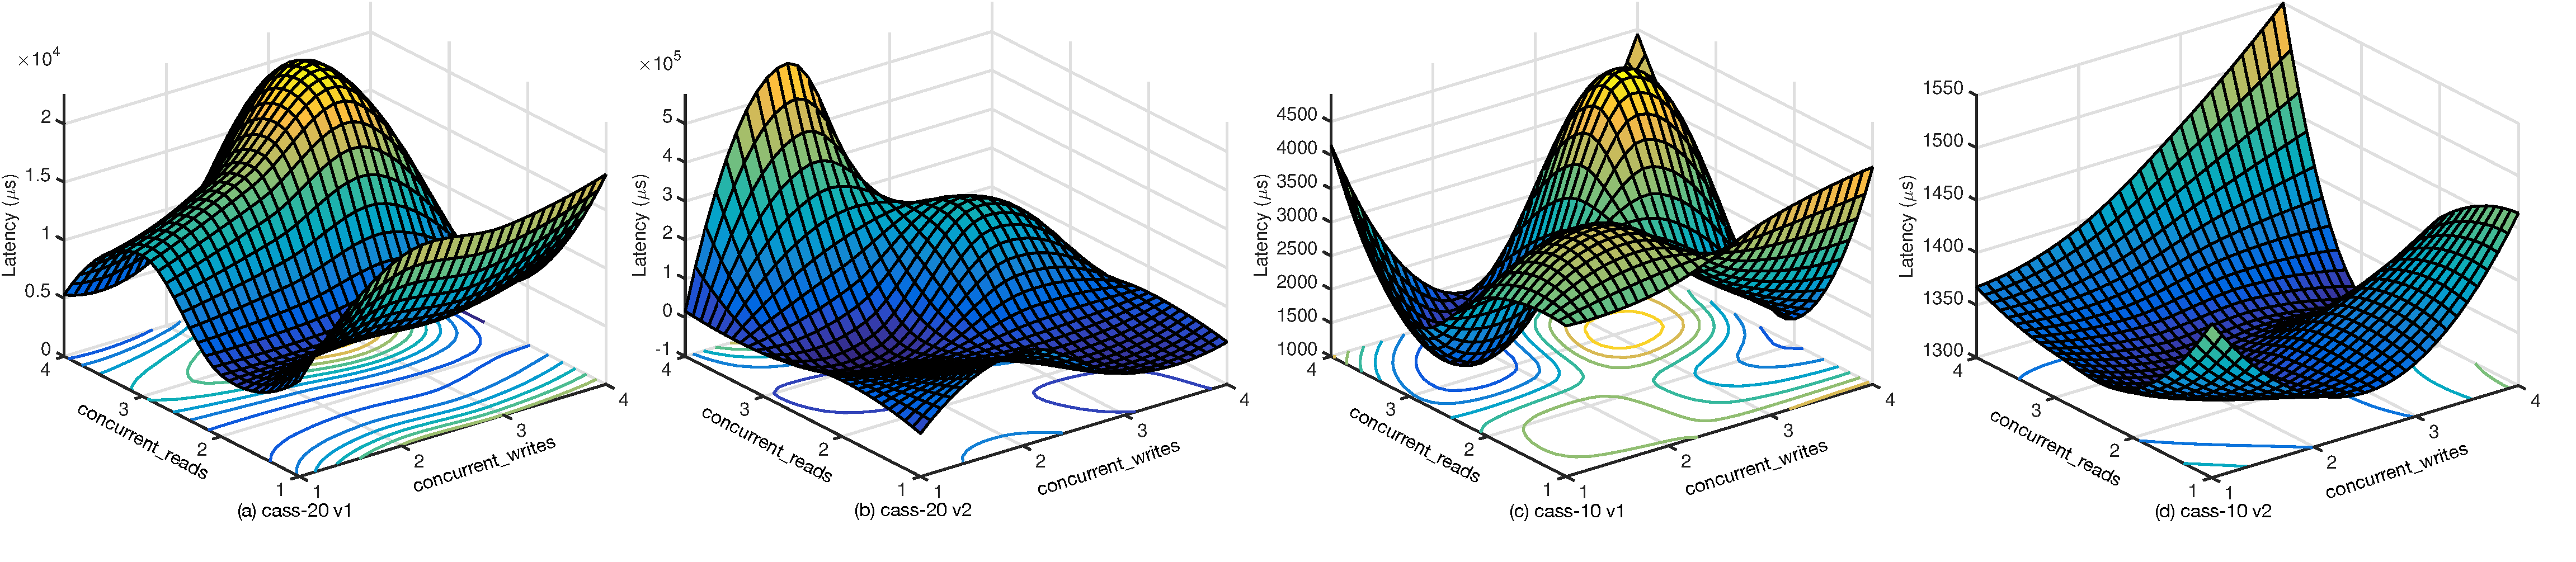
\includegraphics[width=\textwidth]{figures/cass-surfaces-all}
		\caption{The response functions corresponding to the {\sf 2D} subspace of two versions of {\sf cass-10,20}.}
		\label{fig:cass-surf-all}
	\end{center}
\end{figure*}




\newpage
\section{Research Questions and Insights}

The extensive experimental data that we collected to evaluate {\sf TL4CO} could be used to address several research questions. Due to the space limitation, we did not specified the question explicitly in the paper. Instead, here we define the questions and provide evidences based on the results reported in the paper. Here, we only focus on the research questions that we believe are most important for \emph{software engineering} community.

{\noindent \em \textbf{RQ1}: How large is the potential difference and as a result potential impact of a wrong choice of parameter settings?}

We demonstrated for both SPS in Figure 2 (\emph{in the paper}) and for NoSQL systems in Figure \ref{fig:read-latency-hist} and also in Figure \ref{fig:cass-surf-all} that the performance difference between different configurations is significant. The error measures in the experimental results in the paper also demonstrate this large difference. The performance gain between the worst and best settings are measured for each datasets in Table \ref{tab:performance-gain}.

\begin{table}[h]
	\centering
	\caption{Performance gain between best and worst settings.} %The merit function indicates the significant is the set of strongly-interacting parameters that best explains the data. 
	\label{tab:performance-gain}
	\resizebox{0.9\columnwidth}{!}{%
		\begin{threeparttable}
			\begin{tabular}{llccg}
				\toprule
				&\textbf{Dataset} & \multicolumn{1}{c}{\textbf{Best (ms)}}                                                                                       & \multicolumn{1}{c}{\textbf{Worst(ms)}} & \multicolumn{1}{c}{\textbf{Gain (\%)}}                                                                             \\ \midrule
				1  & {\sf wc(6D) }               &       55209          & 3.3172 & 99\%                 \\ \midrule
				2  & {\sf sol(6D) }         &           40499         & 1.2000 & 100\%                  \\ \midrule
				3  & {\sf rs(6D) }           &                34733           & 1.9000 & 99\%              \\ \midrule
				4  & {\sf wc(3D)}            &        94553           & 1.2994 & 100\%            \\ \midrule
				%				5  & {\sf wc+rs }          & \begin{tabular}[c]{@{}l@{}}{\sf 1-max\_spout, 2-splitters,} \\ {\sf 3-counters} \end{tabular}                                                                              & 196 & C4                                \\ \midrule
				%				6  & {\sf wc+sol }         & \begin{tabular}[c]{@{}l@{}}{\sf 1-max\_spout, 2-splitters,} \\ {\sf 3-counters} \end{tabular}                                                                                  & 196 & C4                              \\ \midrule
				%				7  & {\sf wc+wc }        & \begin{tabular}[c]{@{}l@{}}{\sf 1-max\_spout, 2-splitters,} \\ {\sf 3-counters} \end{tabular}                                                                       & 196 & C4                                \\ \midrule
				5  & {\sf wc(5D)}   &       405.5             & 47.387 & 88\%              \\ \midrule
				%				9  & {\sf wc-c1}        & \begin{tabular}[c]{@{}l@{}}{\sf 1-spout\_wait, 2-splitters, }\\ {\sf 3-counters} \end{tabular}                                                                               & 1343 & C1                          \\ \midrule
				%				10 & {\sf wc-c3}      & \begin{tabular}[c]{@{}l@{}}{\sf 1-spout\_wait, 2-splitters,} \\ {\sf 3-counters} \end{tabular}                                                              & 1512 & C3 \\  \midrule
				6  & {\sf cass-10}     &         1.955   & 1.206 & 38\%        \\ \midrule
				7  & {\sf cass-20}      &        40.011    & 2.045 & 95\%        \\ 
				
				\bottomrule
			\end{tabular}
		\end{threeparttable}}
	\end{table}



\colorbox{gray}{
\begin{minipage}{\dimexpr0.88\columnwidth}
Different parameter settings cause very large variance in the performance of the system under test.
\end{minipage}	
}
\vspace{1em}




{\noindent \em \textbf{RQ2}: How does a ``default'' setting compare to the worst and optimum configuration in terms of performance?}

Figure 16 reports the relative performance for the default setting, in terms of throughput and latency with the worst and best configuration as well as the one prescribed by NoSQL experts. As opposed our expectations, a default configuration is worst that majority of other configurations, it performs better than only 10\% of other settings for read operations. However, for write operations the default configurations performs better than half of the other settings. This was expected because Apache Cassandra is designed to be write efficient. Even the configuration that is prescribed by practitioners and NoSQL experts is far from the optimum setting {\sf TL4CO} found after only 100 iterations.

\vspace{1em}
\colorbox{gray}{
	\begin{minipage}{\dimexpr0.88\columnwidth}
		 Default parameter settings perform poorly. The expert's prescription is also far from optimal on individual problem instances.
	\end{minipage}	
}
\vspace{1em}

{\noindent \em \textbf{RQ3}: How is the performance of a configuration optimization on a version when it has been tuned on another version?}

If one makes tuning on a specific version of the system under test, then we would expect it would be optimum for other versions of the system after it has gone under some changes. The results for both SPS and NoSQL in Figures 2 and \ref{fig:cass-surf-all} show that the optimum setting will be different for different versions. We also observed that parameter settings that should work well on average can be particularly inefficient on new versions compared to the best configuration for those versions. In other words, there is a very high variance in the performance of parameter settings. This has been also observed by another study in search-based software engineering community \cite{arcuri2013parameter}. One interesting observations that has not reported previously is that the performance data have correlations among different versions.

\vspace{1em}
\colorbox{gray}{
	\begin{minipage}{\dimexpr0.88\columnwidth}
		 Tuned parameters can improve upon default values on average, but they are far from optimal on individual problem instances.
	\end{minipage}	
}
\vspace{1em}

{\noindent \em \textbf{RQ4}: How much can transfer learning improve tuning with a larger number of observations from other versions?}

The larger the training set is, the more accurate the model predictions will likely be. In the context of configuration tuning, carrying over a larger observation set will result in better tuning, but it would be more expensive to carry out the optimization process as we have shown in Section 4.6. The results in Figure 18(b) and Figure 19(b) show that although the models become more accurate slightly, the gain in performance tuning does not pay off the costs.

\vspace{1em}
\colorbox{gray}{
	\begin{minipage}{\dimexpr0.88\columnwidth}
		 Although transferring more observations improves performance and reduce the entropy, the improvement is low.
	\end{minipage}	
}


\bibliographystyle{abbrv}
%\bibliography{sigproc}  % sigproc.bib is the name of the Bibliography in this case
%\footnotesize
\bibliography{sigproc.bib}


\end{document}
